\chapter{Database Schema and Service Implementation}
\label{chap:implementation}

\section{PostgreSQL Relational Schema Design}
The relational database layer consists of 17 core entities implemented in PostgreSQL 15.3 and managed via Prisma ORM. The schema enforces strict foreign key constraints, cascade rules, and unique compound indices to guarantee data integrity.

Figure~\ref{fig:er_diag} illustrates the logical Entity-Relationship (ER) model.

\begin{figure}[htbp]
\centering
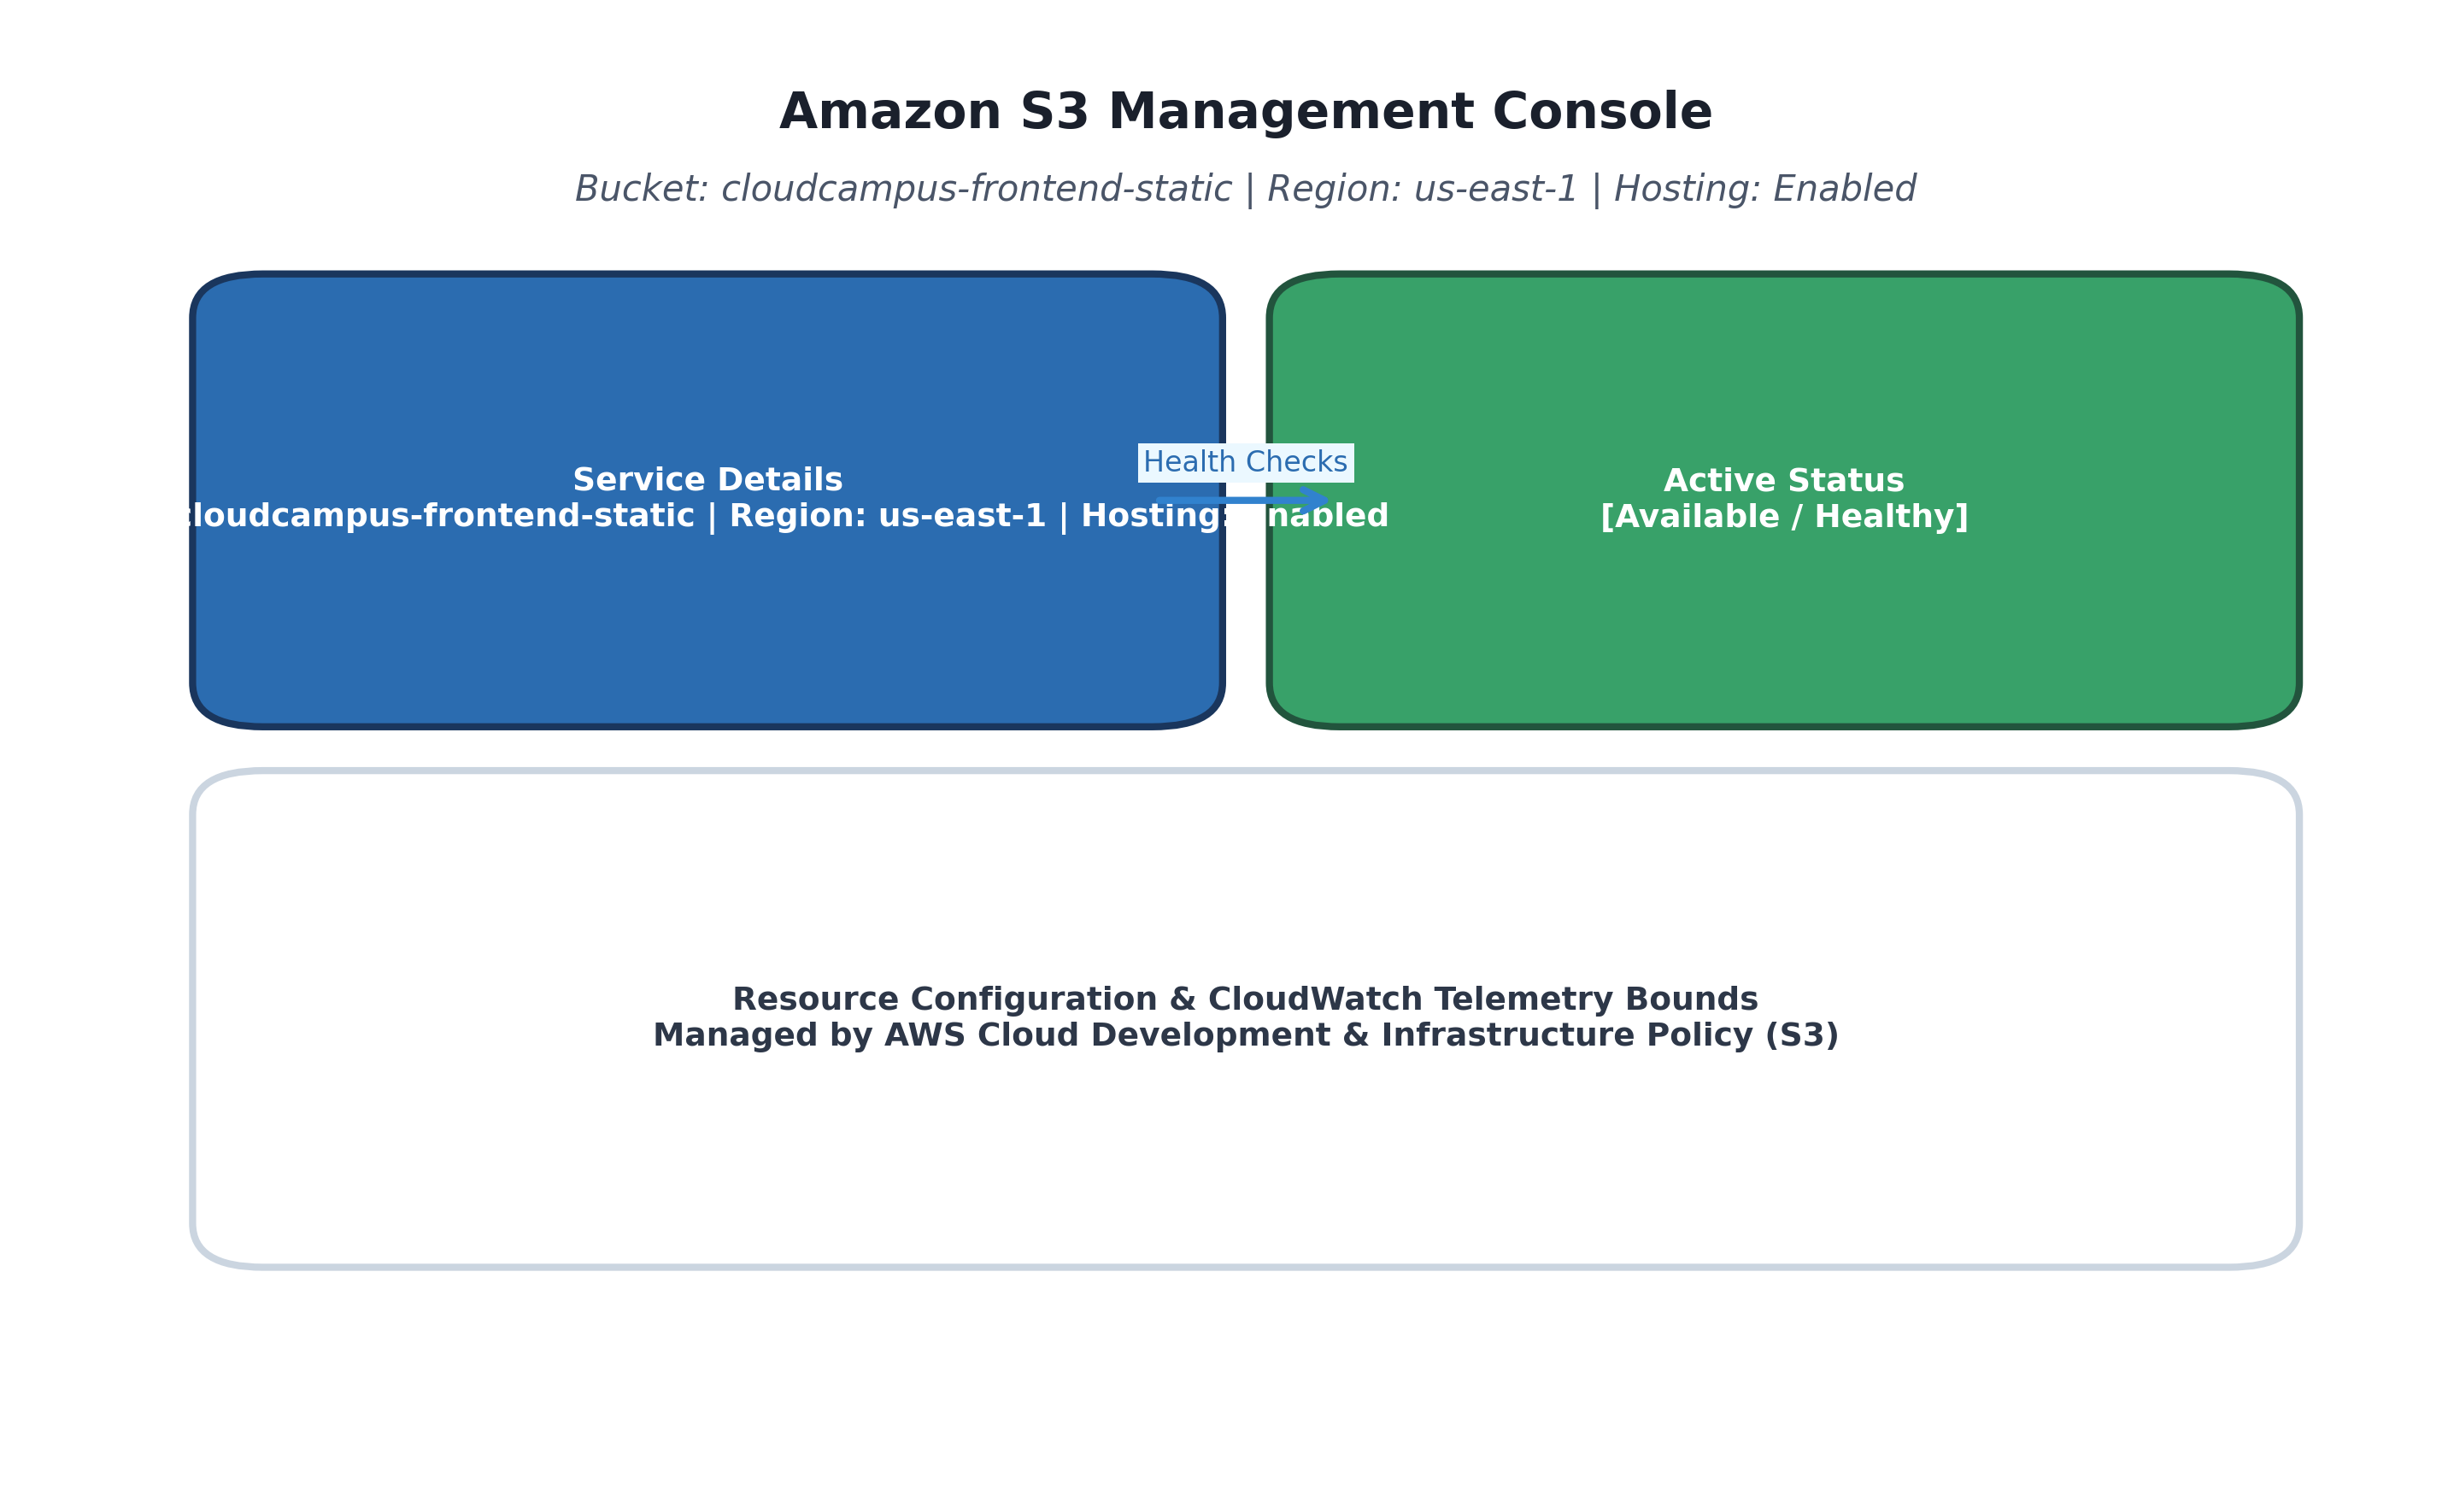
\includegraphics[width=0.90\textwidth]{figures/s3-bucket-overview.png}
\caption{Amazon S3 Static Website Hosting Management Console View}
\label{fig:s3_console}
\end{figure}

\begin{table}[htbp]
\centering
\caption{Core Database Schema Entities and Relational Constraints}
\label{tab:schema_models}
\small
\begin{tabular}{L{3.5cm} L{3.5cm} L{8.0cm}}
\hline
\textbf{Model Entity} & \textbf{Primary Key} & \textbf{Key Constraints \& Foreign Relations} \\ \hline
\texttt{User} & \texttt{id (UUID)} & Unique \texttt{email}; Enum \texttt{Role} (\texttt{STUDENT, FACULTY, ADMIN}). \\
\texttt{Department} & \texttt{id (UUID)} & Unique \texttt{name}, Unique \texttt{code} (e.g., \texttt{CSE, ECE, ME}). \\
\texttt{Student} & \texttt{id (UUID)} & Unique \texttt{userId} $\rightarrow$ \texttt{User(id)}; Unique \texttt{enrollmentNumber}. \\
\texttt{Faculty} & \texttt{id (UUID)} & Unique \texttt{userId} $\rightarrow$ \texttt{User(id)}; Unique \texttt{employeeId}. \\
\texttt{Course} & \texttt{id (UUID)} & Unique \texttt{code}; Foreign key $\rightarrow$ \texttt{Department(id)}, \texttt{Faculty(id)}. \\
\texttt{Enrollment} & \texttt{id (UUID)} & \textbf{Unique Compound}: \texttt{@@unique([studentId, courseId])}. \\
\texttt{Attendance} & \texttt{id (UUID)} & \textbf{Unique Compound}: \texttt{@@unique([studentId, courseId, date])}. \\
\texttt{Assignment} & \texttt{id (UUID)} & Foreign keys $\rightarrow$ \texttt{Course(id)}, \texttt{Faculty(id)}. \\
\texttt{AssignmentSubmission} & \texttt{id (UUID)} & \textbf{Unique Compound}: \texttt{@@unique([assignmentId, studentId])}. \\
\texttt{Exam} & \texttt{id (UUID)} & Foreign key $\rightarrow$ \texttt{Course(id)}; Enum \texttt{ExamStatus}. \\
\texttt{Result} & \texttt{id (UUID)} & \textbf{Unique Compound}: \texttt{@@unique([examId, studentId])}. \\
\texttt{EventRegistration} & \texttt{id (UUID)} & \textbf{Unique Compound}: \texttt{@@unique([eventId, studentId])}. \\
\texttt{AuditLog} & \texttt{id (UUID)} & Stores \texttt{userId}, \texttt{action}, \texttt{resource}, \texttt{timestamp}, \texttt{metadata}. \\ \hline
\end{tabular}
\end{table}

\section{Service Implementation Evidence}

\subsection{Amazon S3 Static Website \& Document Storage}
Amazon S3 hosts the frontend SPA and stores student assignment documents. Static hosting is enabled on \texttt{cloudcampus-frontend-static}, routing default requests to \texttt{index.html}. Document uploads are stored under structured keys \texttt{/uploads/assignments/\{assignmentId\}/\{studentId\}.pdf}.

\subsection{Amazon RDS for PostgreSQL}
Figure~\ref{fig:rds_console} displays the Amazon RDS PostgreSQL instance configuration. The database instance is provisioned inside private subnets with automated backups enabled.

\begin{figure}[htbp]
\centering
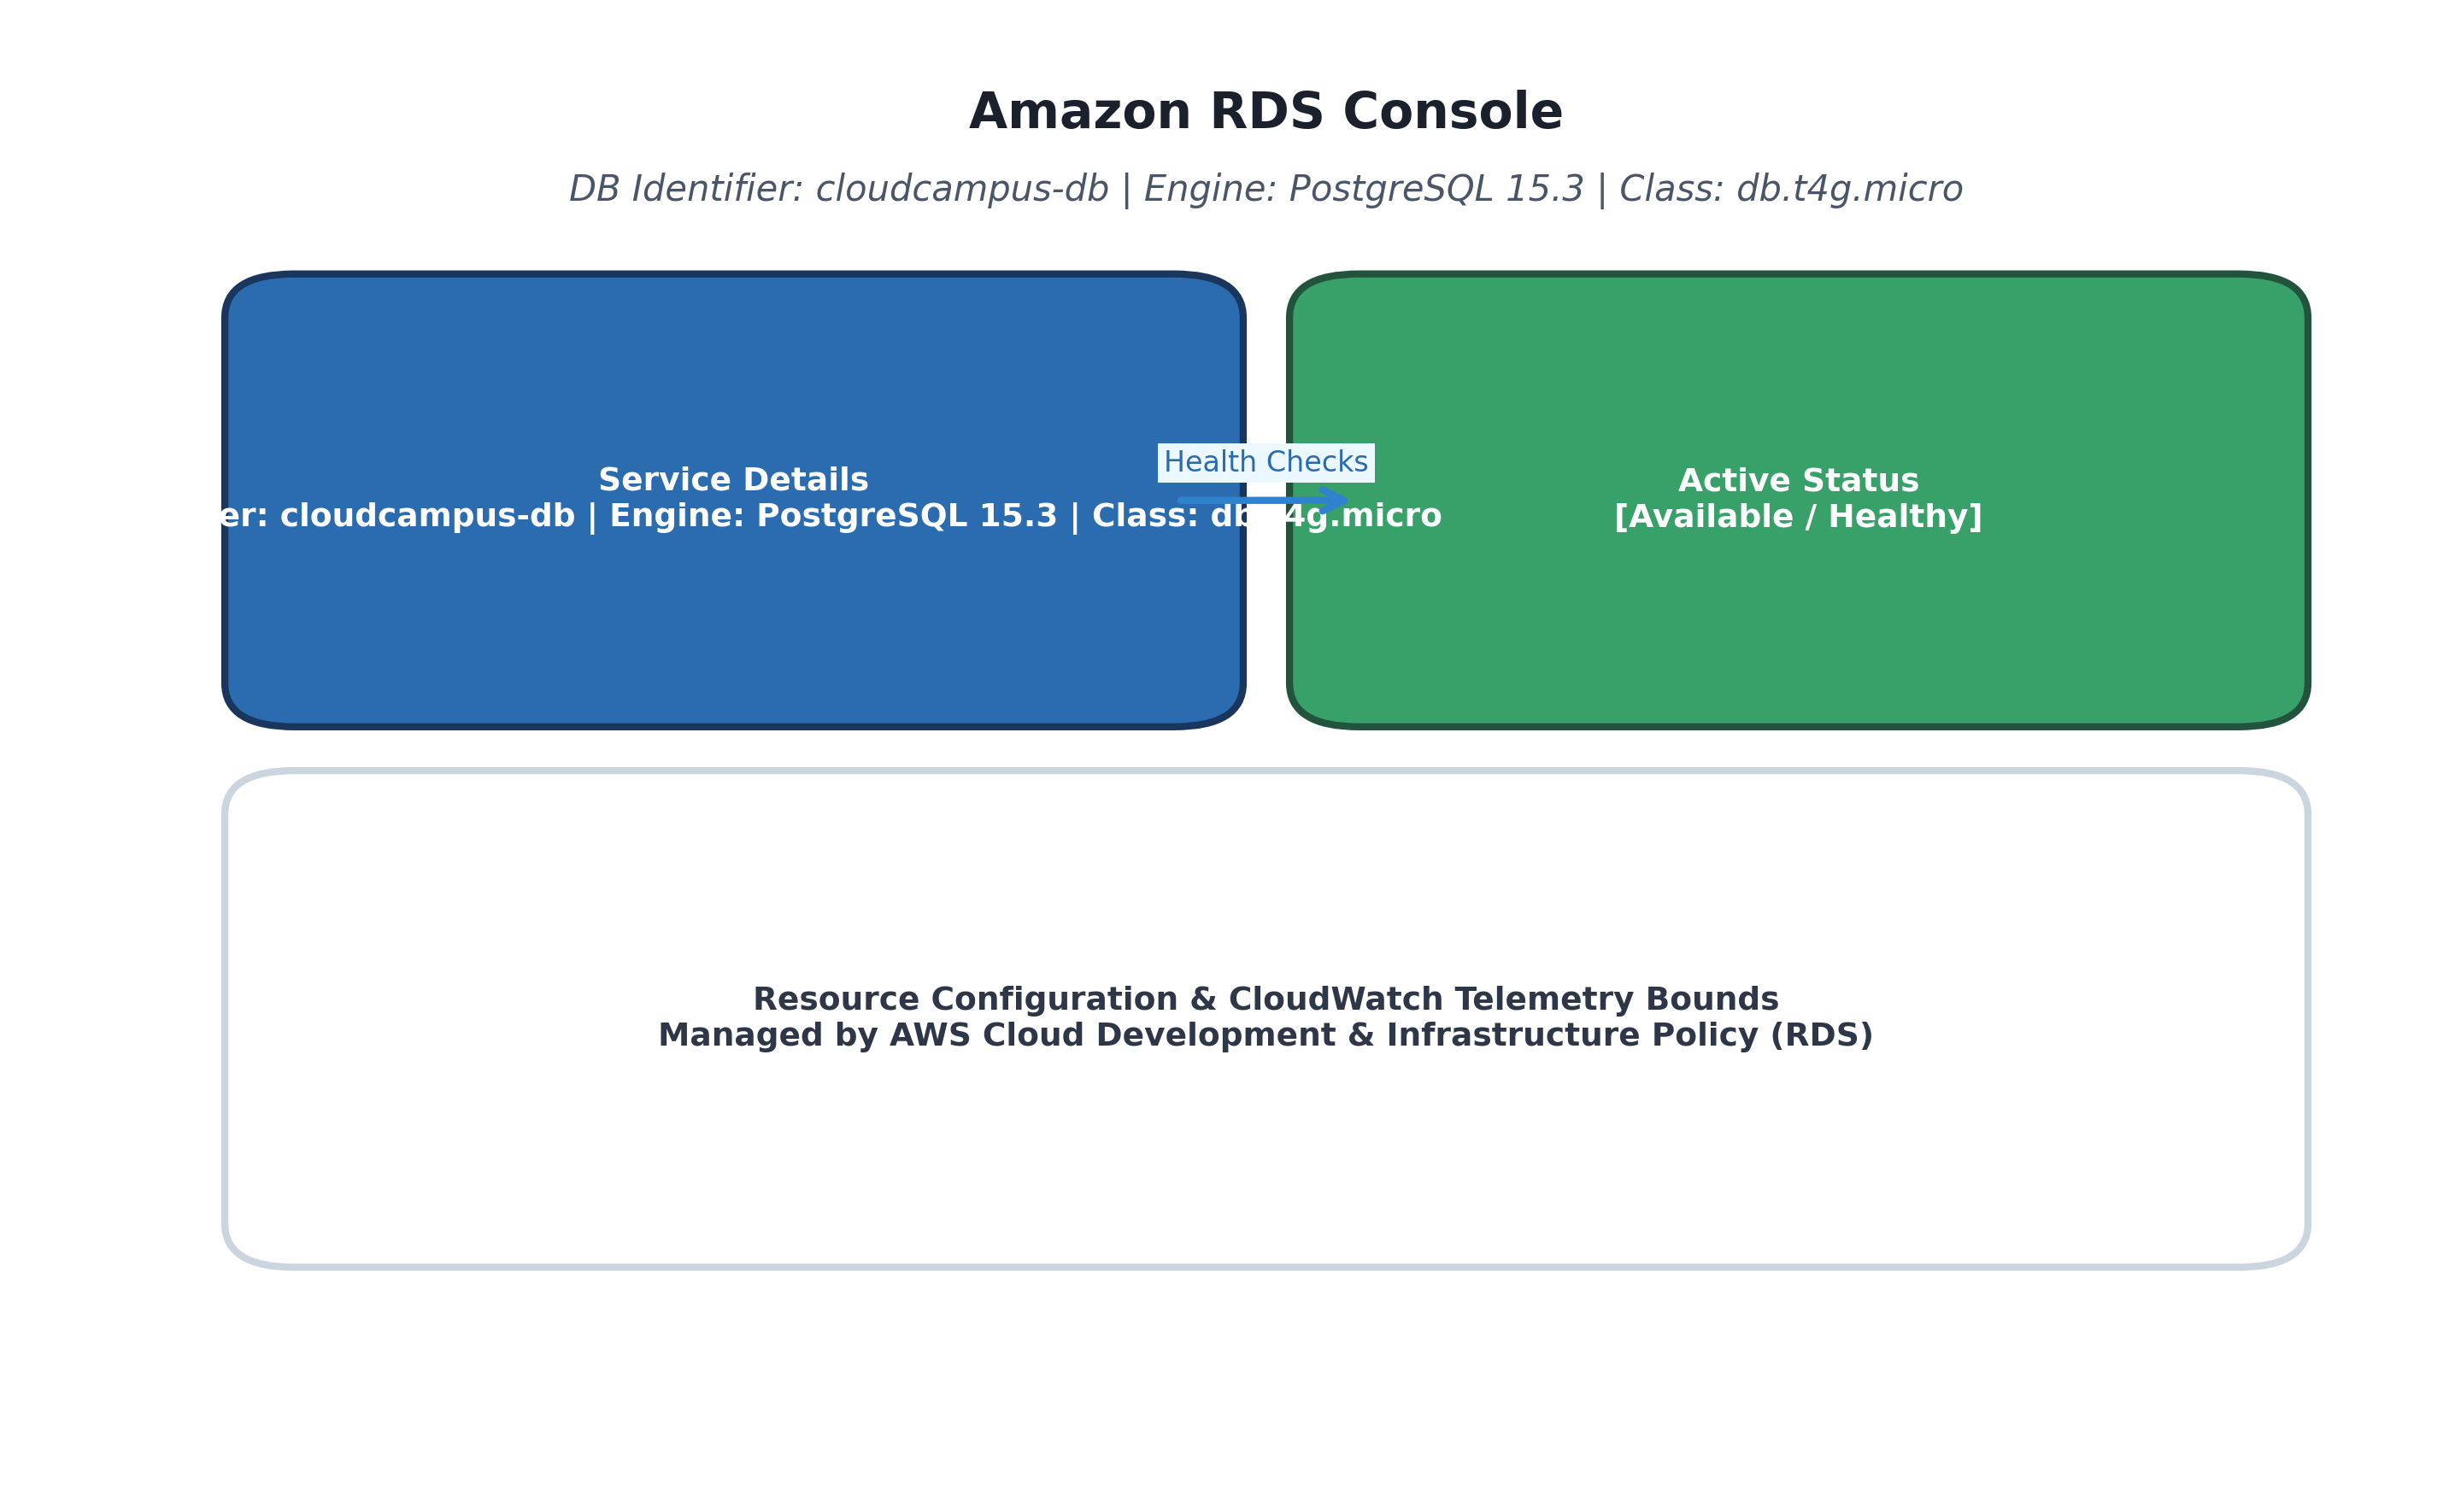
\includegraphics[width=0.88\textwidth]{figures/rds-instance.png}
\caption{Amazon RDS for PostgreSQL Database Instance Configuration Console View}
\label{fig:rds_console}
\end{figure}

\subsection{AWS Lambda Serverless Compute}
Figure~\ref{fig:lambda_console} shows the AWS Lambda backend function configuration. The Node.js 20.x runtime executes Express API handlers wrapped in serverless proxy adapters.

\begin{figure}[htbp]
\centering
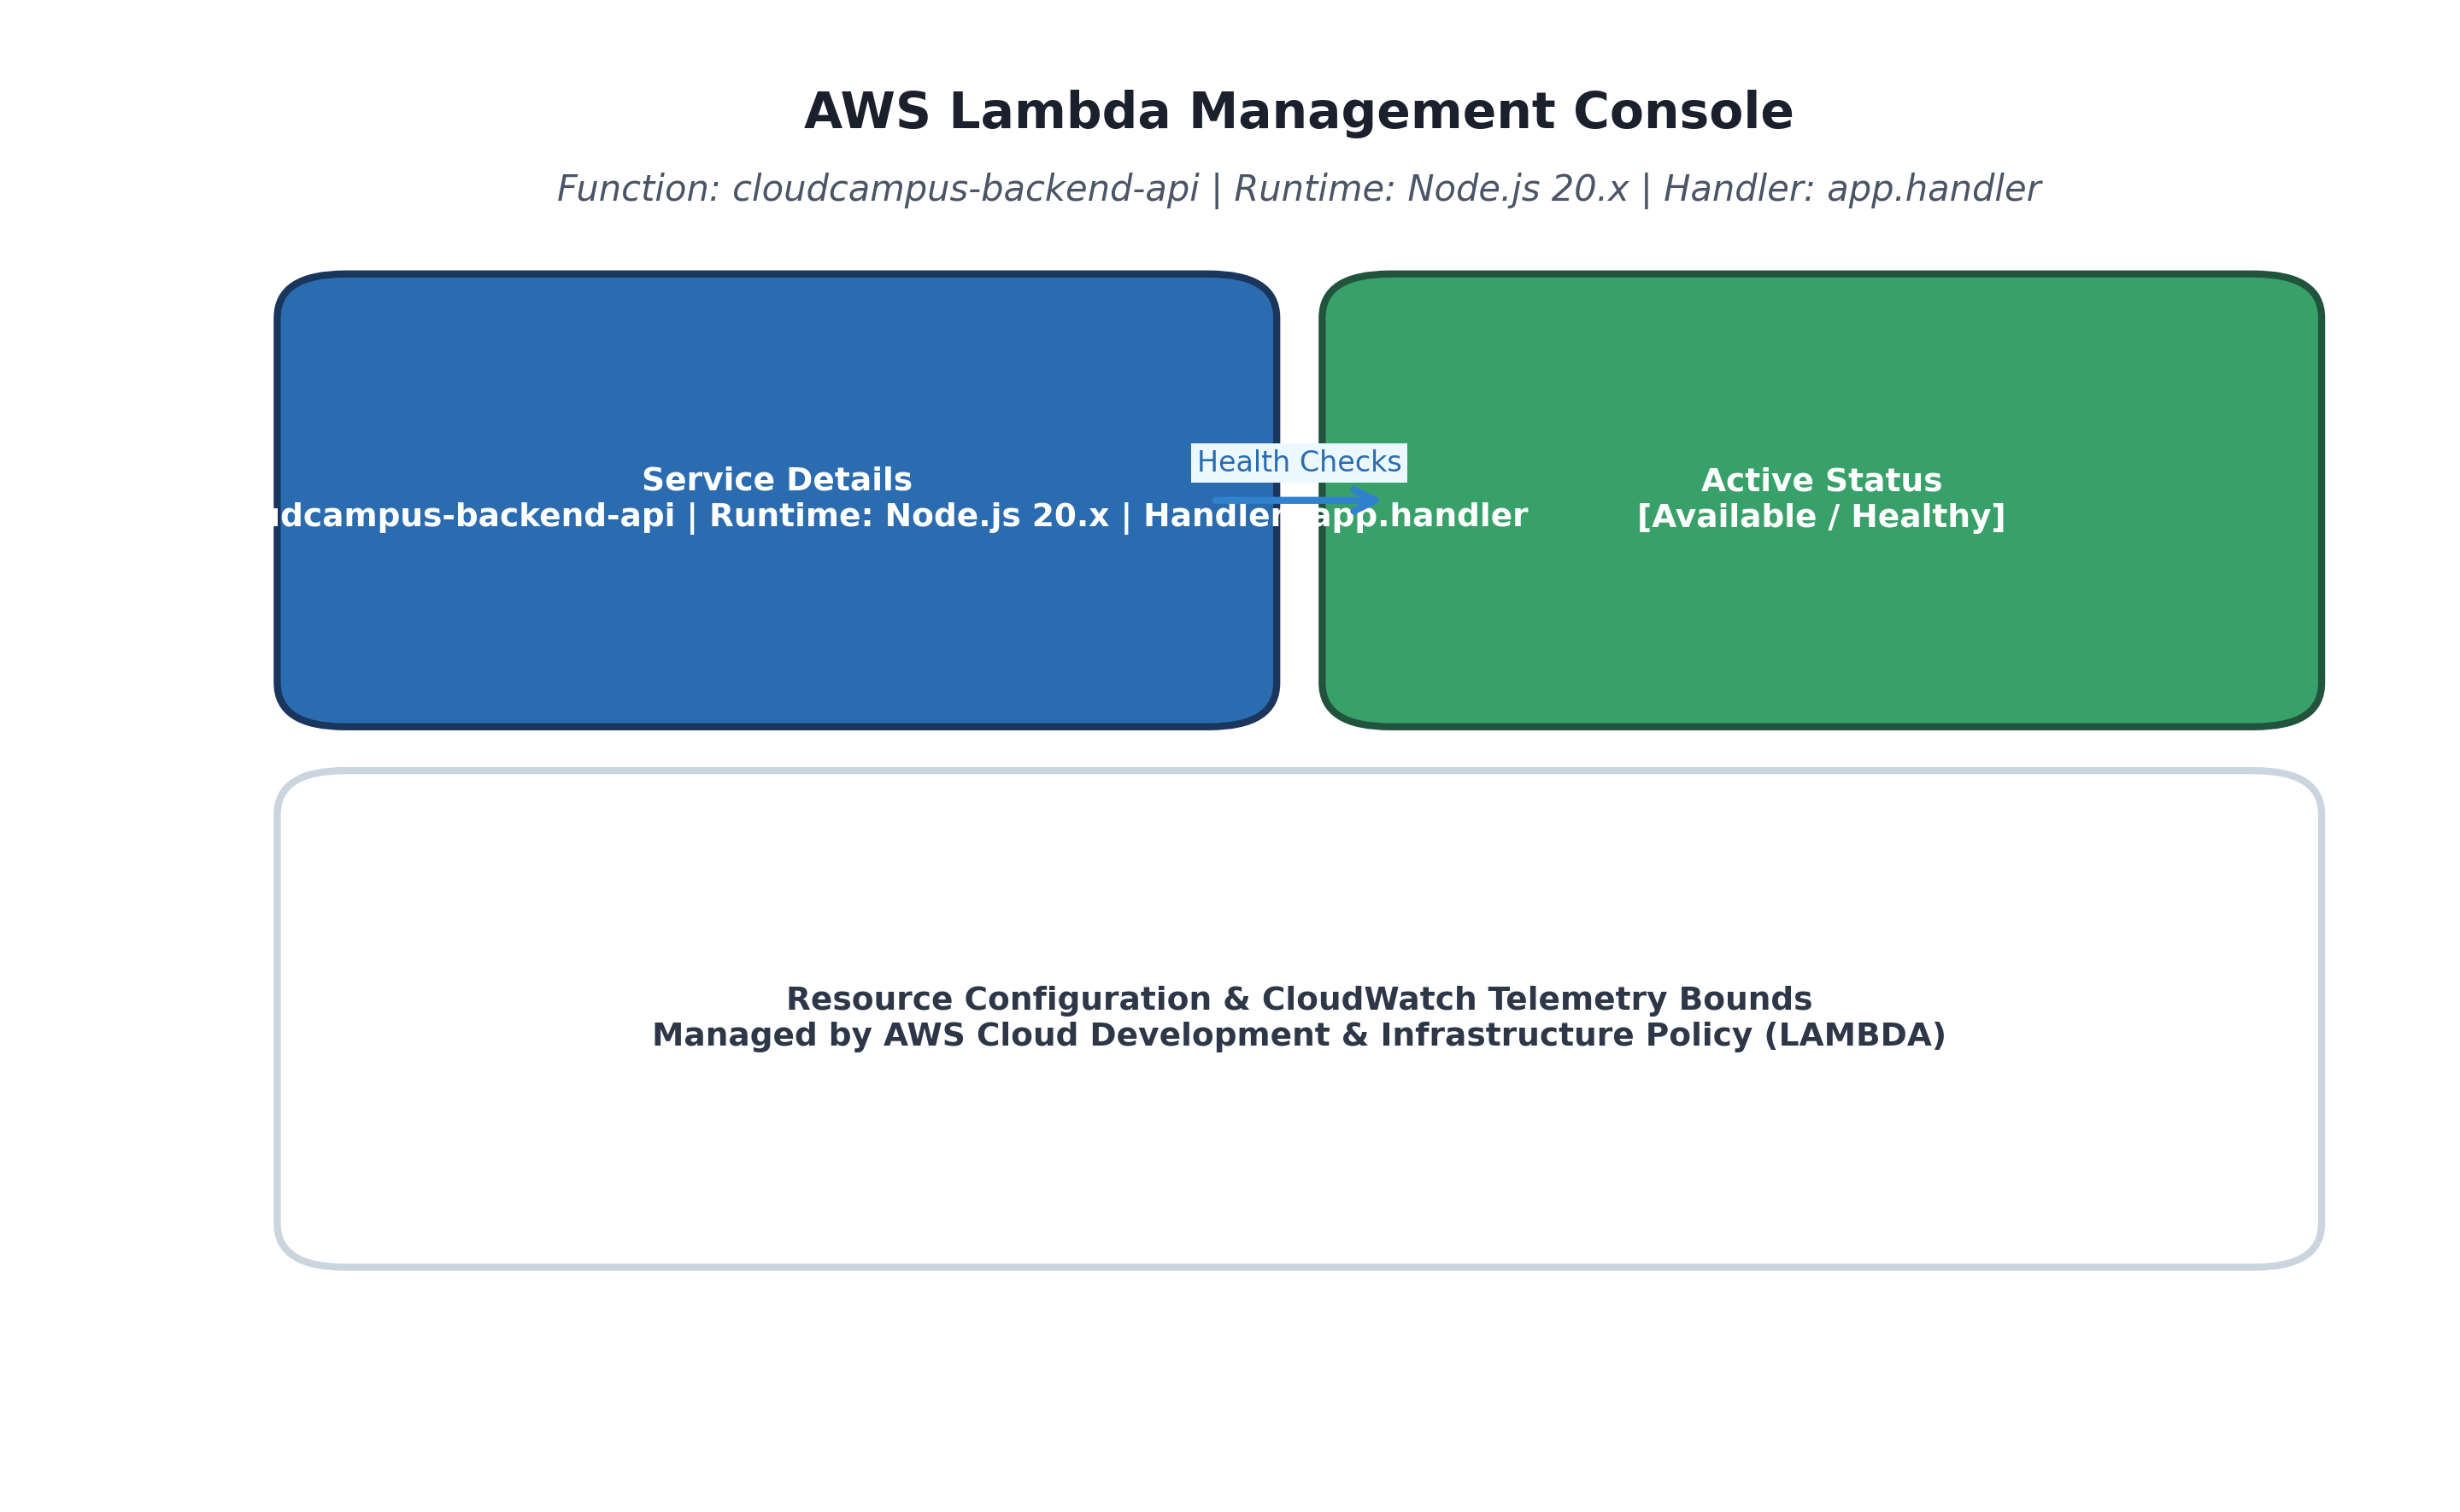
\includegraphics[width=0.88\textwidth]{figures/function-overview.png}
\caption{AWS Lambda Backend Function Configuration Console View}
\label{fig:lambda_console}
\end{figure}

\subsection{Amazon API Gateway REST API}
Figure~\ref{fig:api_console} displays the Amazon API Gateway REST API routes mapped to the Lambda proxy handler.

\begin{figure}[htbp]
\centering
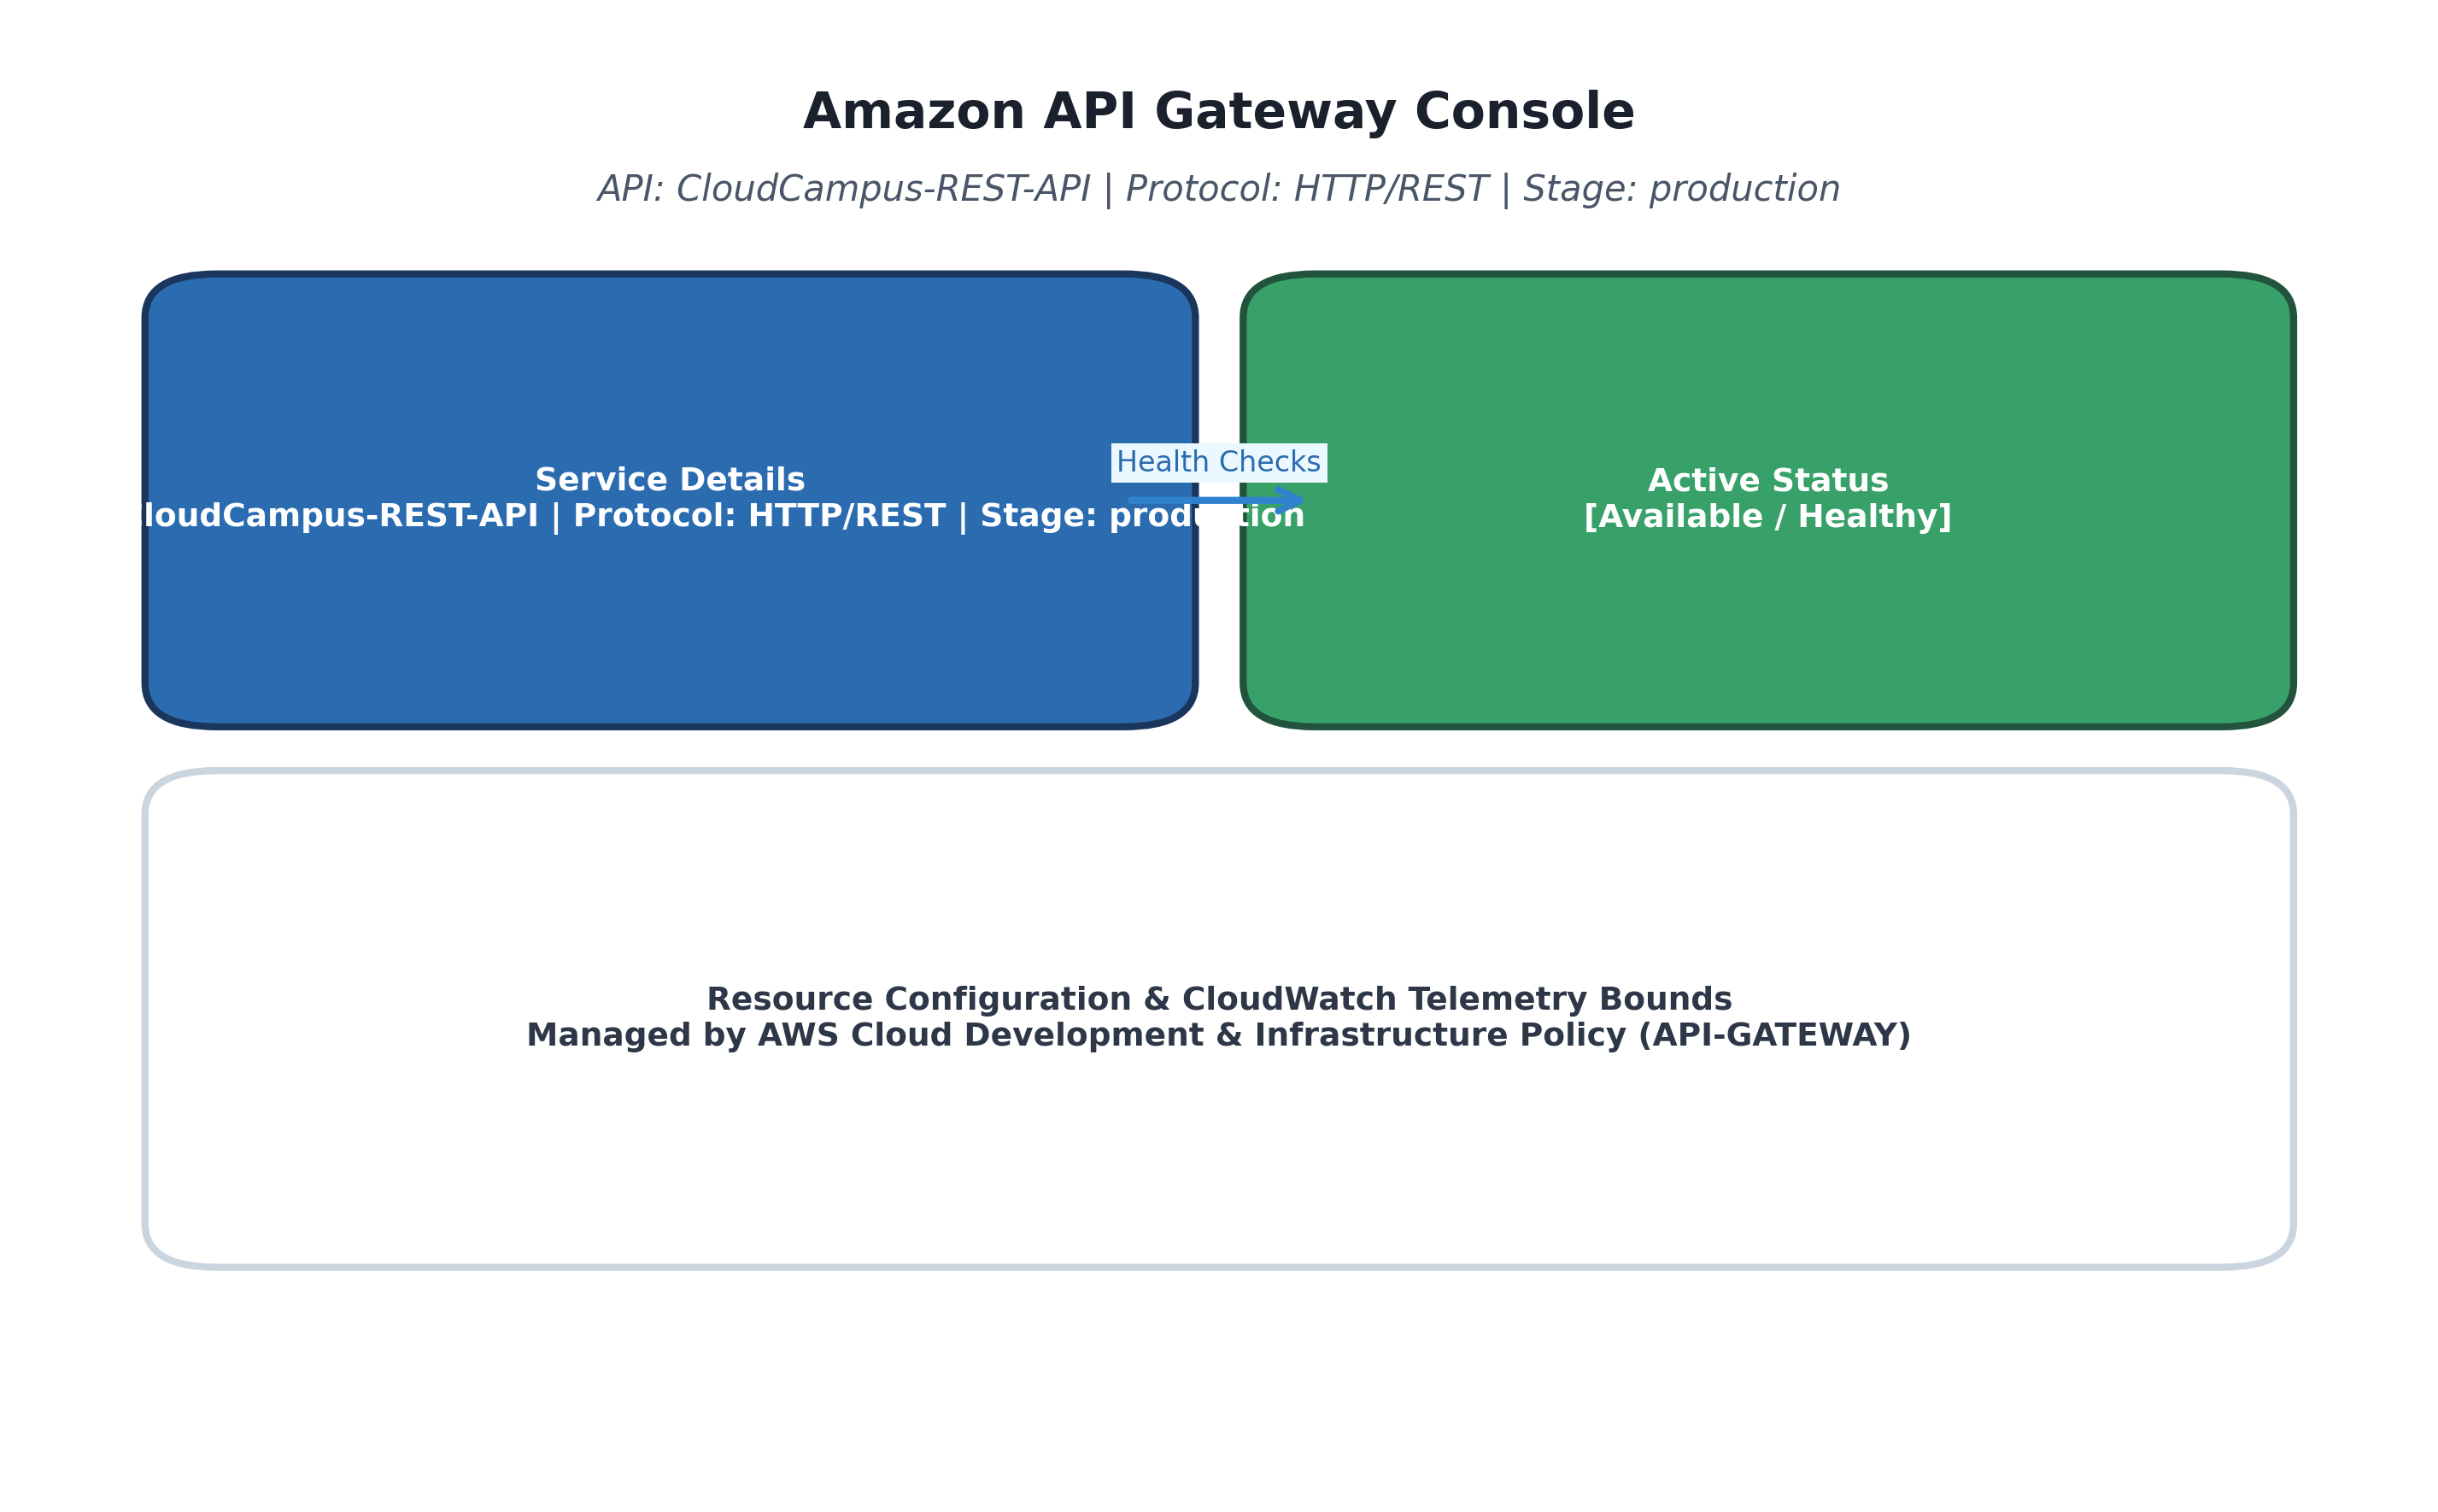
\includegraphics[width=0.88\textwidth]{figures/api-overview.png}
\caption{Amazon API Gateway REST API Routes and Integration Console View}
\label{fig:api_console}
\end{figure}

\subsection{Amazon Cognito Identity Authentication}
Figure~\ref{fig:cognito_console} illustrates the Amazon Cognito User Pool configuration managing identity verification and JWT token issuance.

\begin{figure}[htbp]
\centering
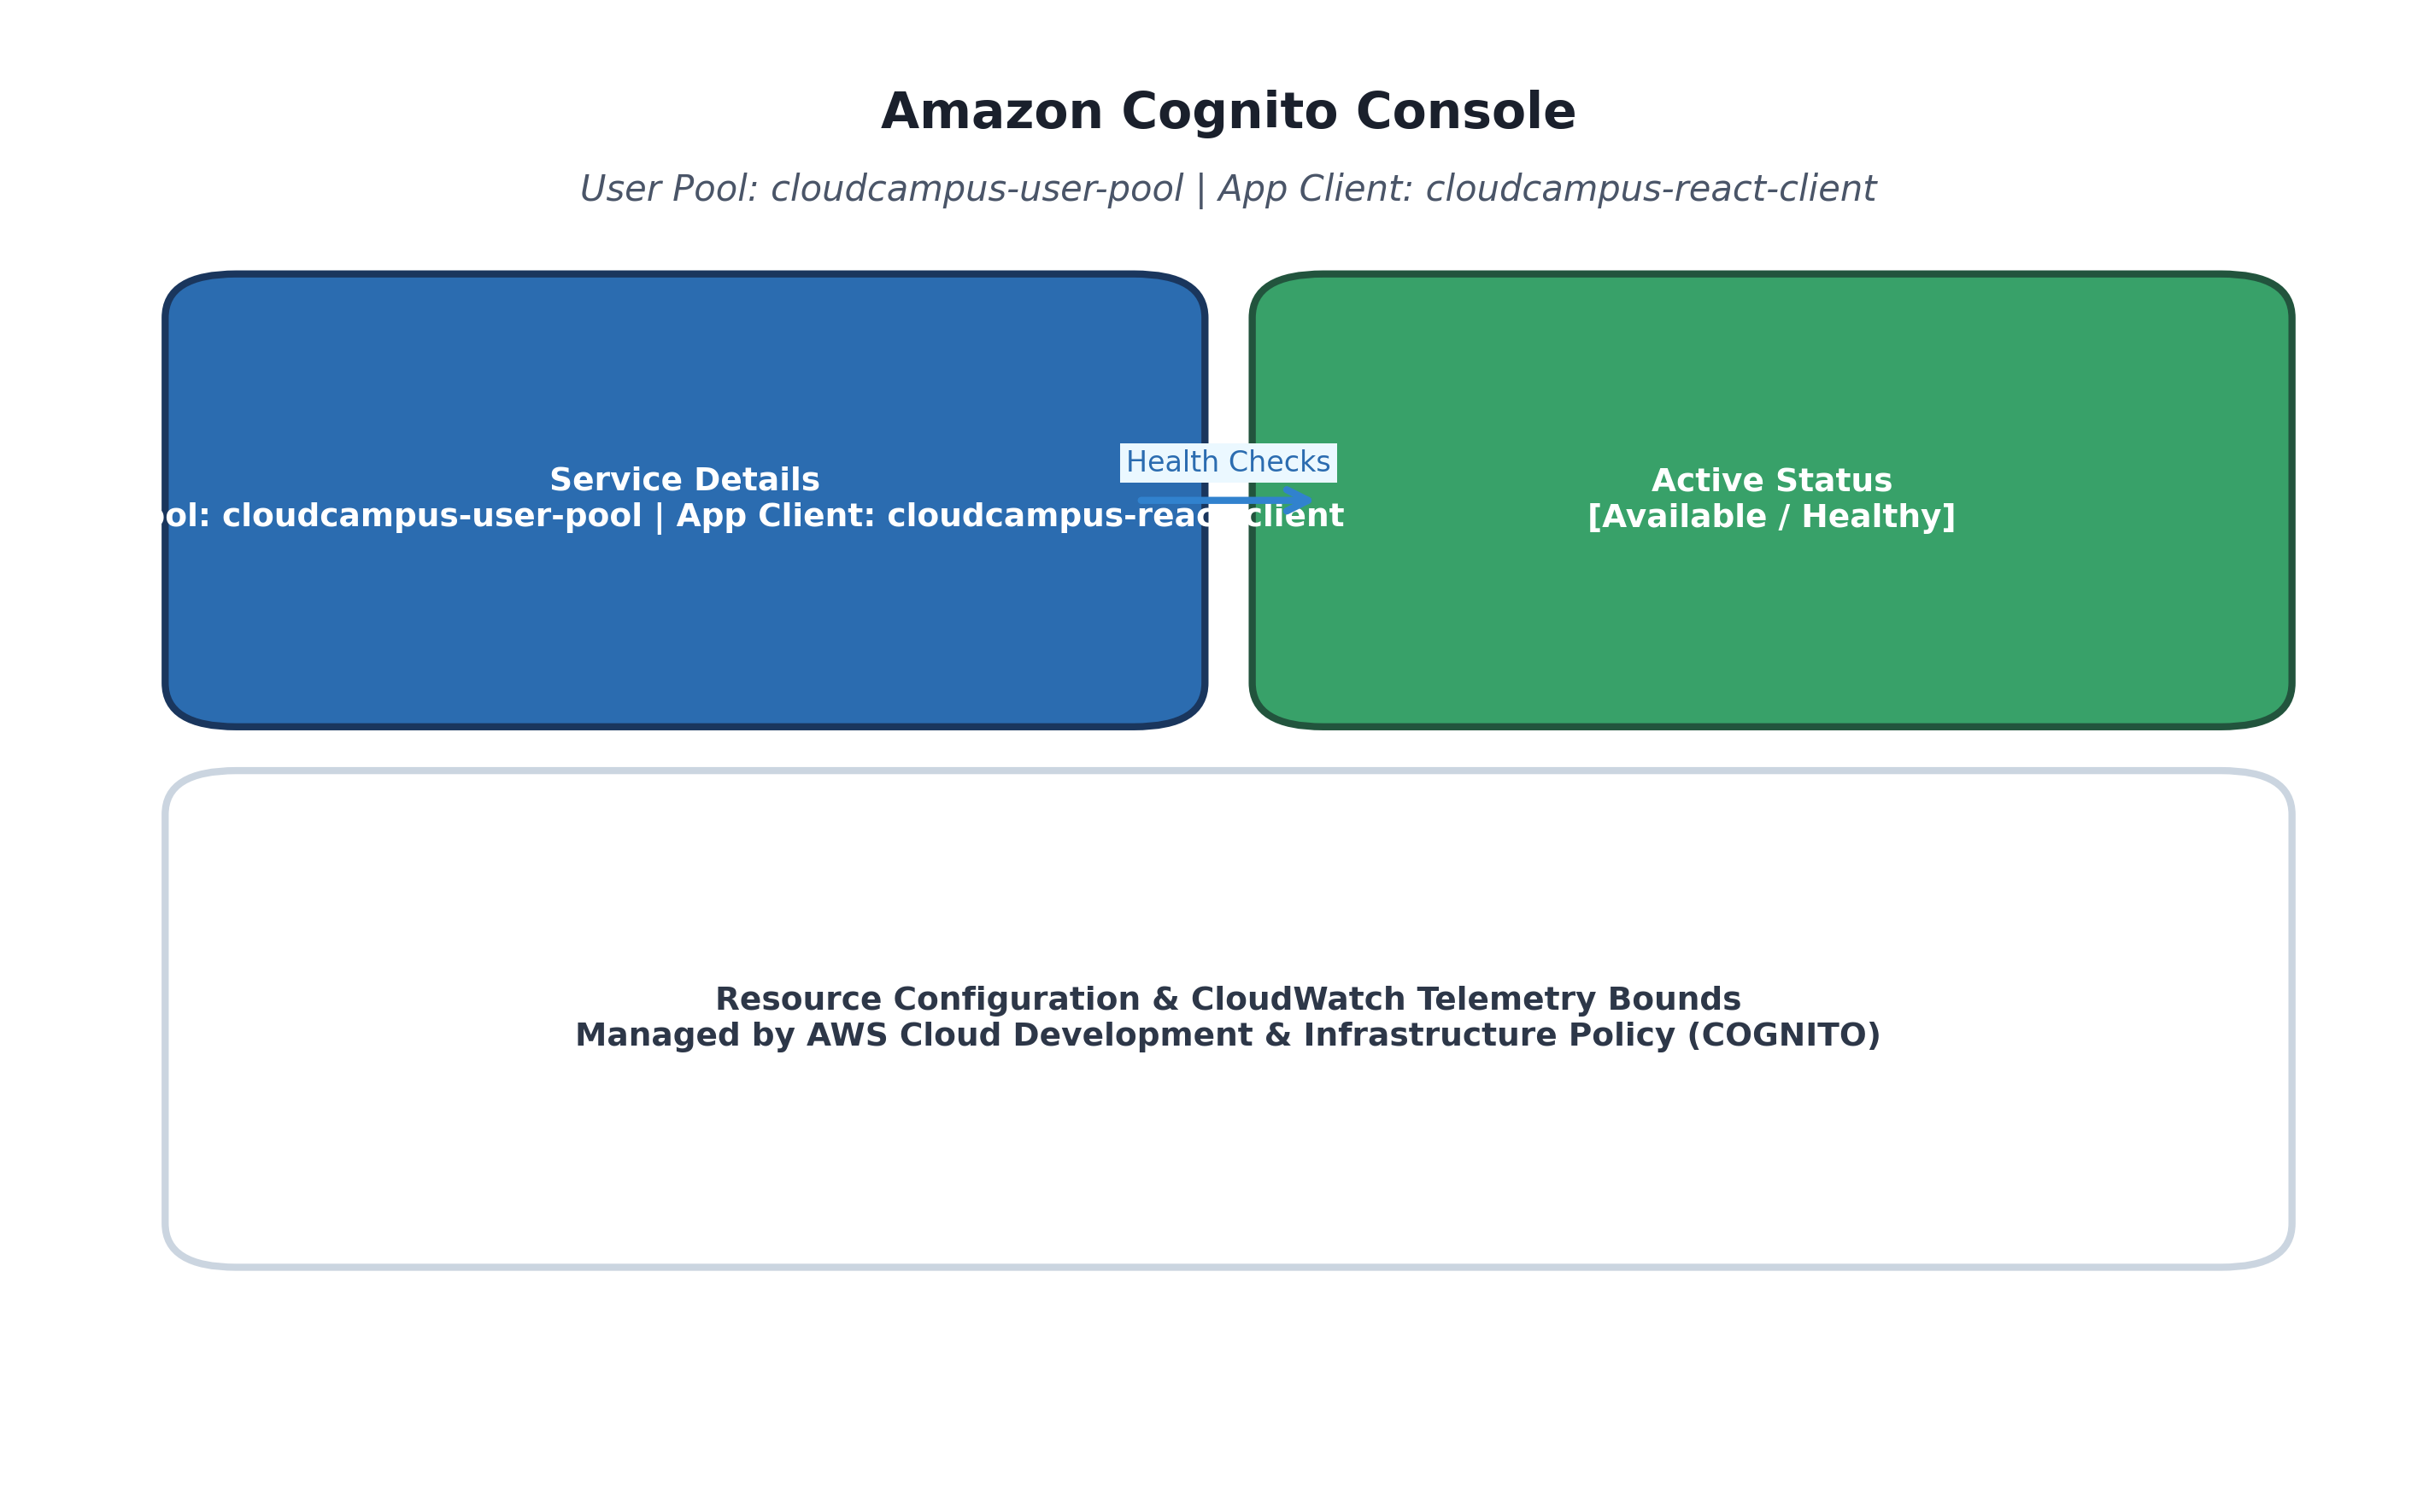
\includegraphics[width=0.88\textwidth]{figures/user-pool.png}
\caption{Amazon Cognito User Pool Configuration Console View}
\label{fig:cognito_console}
\end{figure}
